
Relembrando, o objetivo deste trabalho é criar uma biblioteca no MATLAB que permita a resolução de problemas de otimização de trajetória de maneira facilitada, de forma que o usuário precise apenas modelar o problema, sem a necessidade de implementar a lógica da solução numérica. Para isso, é necessário que a biblioteca forneça uma interface de dados, de modo a permitir que o usuário entre com a modelagem do seu problema. Além disso, deve-se implementar a colocação trapezoidal como método de solução.

Para validação da implementação a ser realizada, foram implementadas as soluções para alguns problemas exemplos. Tais problemas incluem o estudo de otimização de trajetória de um movimento simples em uma dimensão e braquistócrona, que são problemas clássicos na literatura de otimização de trajetórias, e o estudo de otimização de trajetória de subida de eVTOL em \cite{costa_otimizacao_2023}, o qual utiliza o software PSOPT citado na Seção \ref{sec:rev-bibliografica}.

\section{Interface de Dados}
\label{sec:interface-dados}

Diferente dos softwares OptimTraj \cite{kelly_optimtraj_2022} e PSOPT \cite{becerra_psopt_2022}, a implementação será realizada utilizando uma abordagem de POO, com uma classe MATLAB principal que conterá métodos para a configuração do problema e cálculo da solução. Além da classe principal, a biblioteca contará com funções auxiliares para cálculo da colocação trapezoidal e manipulação de dados.

Os arquivos da biblioteca, assim como os exemplos de uso, estão disponíveis no repositório \cite{simplicio_hsimpliciotg-ita_2024}, e serão descritos na sequência. Para maior clareza, inicialmente será apresentada a classe principal, de modo que será possível entender a estrutura de dados e a lógica de funcionamento da biblioteca. Em seguida, serão apresentadas as funções auxiliares.

\subsection{\texttt{TrajectoryProblem.m}}
\label{subsec:classe-trajectoryproblem}

A classe \texttt{TrajectoryProblem} é a classe principal da biblioteca, e contém métodos para a configuração do problema e cálculo da solução. A classe conta com um construtor, que inicializa os parâmetros e variáveis necessárias para a resolução do problema com valores padrão, e métodos para a configuração dos limites e objetivo do problema, além de um método para a solução numérica do problema.

Dentre os métodos disponíveis, alguns são obrigatórios, ou seja, são necessários para a resolução de qualquer problema, e outros são opcionais, podendo ser utilizados ou não dependendo da necessidade do problema em questão, como pode ser visto na Figura \ref{fig:trajectoryproblem-methods}.

\begin{figure}[H]
    \centering
    \begin{subfigure}{0.6\linewidth}
    \centering
        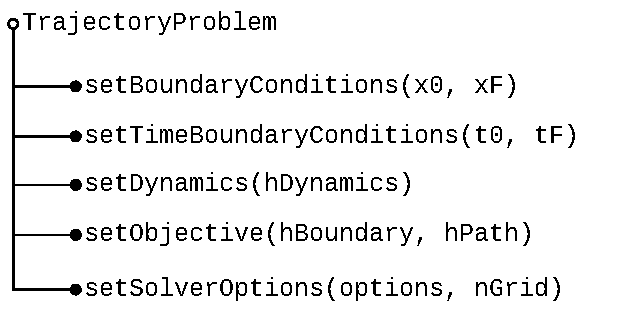
\includegraphics[width=\textwidth]{Cap3/figuras/TrajectoryProblem-mandatory.pdf}
        \caption{Métodos obrigatórios}
    \end{subfigure}
    \hfill
    \begin{subfigure}{0.7\linewidth}
    \centering
        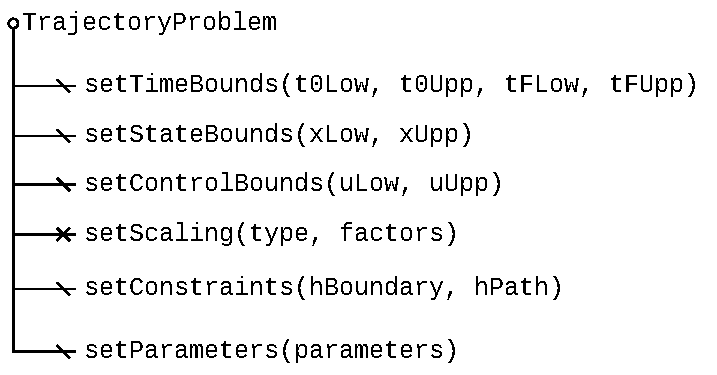
\includegraphics[width=\textwidth]{Cap3/figuras/TrajectoryProblem-optional.pdf}
        \caption{Métodos opcionais}
    \end{subfigure}
    \caption{Métodos da classe \texttt{TrajectoryProblem}}
    \label{fig:trajectoryproblem-methods}
\end{figure}

Além disso, há também métodos auxiliares para a verificação e validação do problema, assim como métodos privados, utilizados internamente pela classe, como pode ser visto na Figura \ref{fig:trajectoryproblem-auxiliar}.

\begin{figure}[H]
    \centering
    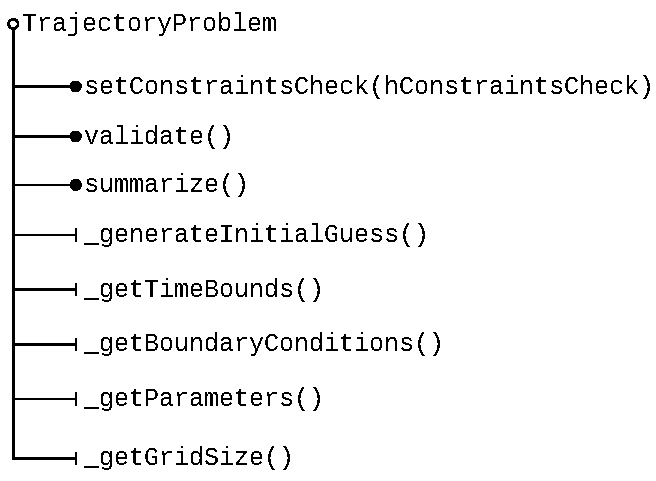
\includegraphics[width=0.64\textwidth]{Cap3/figuras/TrajectoryProblem-auxiliar.pdf}
    \caption{Métodos auxiliares da classe \texttt{TrajectoryProblem}}
    \label{fig:trajectoryproblem-auxiliar}
\end{figure}

Por fim, há o método para a solução do problema com a colocação trapezoidal, apresentado na Figura \ref{fig:trajectoryproblem-solve}, o qual retorna um \texttt{array} de \texttt{structures}, com a solução do problema obtida em cada iteração, além de informações adicionais relacionadas a elas, como apresentado na Figura \ref{fig:solution}.

\begin{figure}[H]
    \centering
    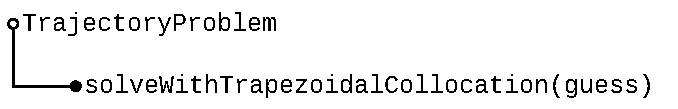
\includegraphics[width=0.66\textwidth]{Cap3/figuras/TrajectoryProblem-solve.pdf}
    \caption{Método para a solução do \texttt{TrajectoryProblem} com a colocação trapezoidal}
    \label{fig:trajectoryproblem-solve}
\end{figure}

\begin{figure}[H]
    \centering
    \begin{subfigure}{0.49\linewidth}
    \centering
        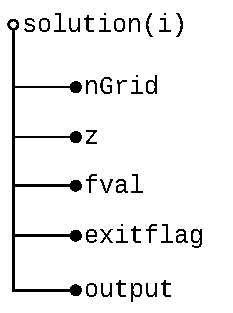
\includegraphics[width=0.45\textwidth]{Cap3/figuras/TrajectoryProblem-solution.pdf}
    \end{subfigure}
    \hfill
    \begin{subfigure}{0.49\linewidth}
    \centering
        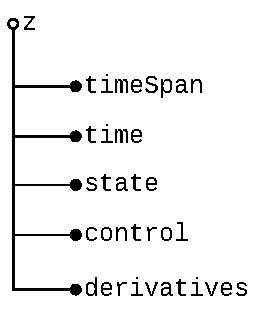
\includegraphics[width=0.52\textwidth]{Cap3/figuras/TrajectoryProblem-solution-z.pdf}
    \end{subfigure}
    \caption{Formato da \texttt{structure} \texttt{solution}}
    \label{fig:solution}
\end{figure}

Na sequência, serão apresentados os métodos da classe, descrevendo sua funcionalidade e uso. O código fonte pode ser encontrado no anexo \ref{sec:codigo-trajectoryproblem}.

\subsubsection{\texttt{.setBoundaryConditions(x0, xF)}}
\label{subsubsec:setboundaryconditions}

Este método recebe como argumentos as condições de contorno do estado do problema, passadas como vetores coluna, os valida e os atribui às propriedades \texttt{x0} e \texttt{xF} da classe.


\subsubsection{\texttt{.setTimeBoundaryConditions(t0, tF)}}
\label{subsubsec:settimeboundaryconditions}

Este método recebe como argumentos os limites de tempo do problema, passados como escalares, os valida e os atribui às propriedades \texttt{t0} e \texttt{tF} da classe.

\subsubsection{\texttt{.setTimeBounds(t0Low, t0Upp, tFLow, tFUpp)}}
\label{subsubsec:settimebounds}

Este método recebe como argumentos os limites de tempo do problema, passados como escalares, os valida e os atribui às propriedades \texttt{t0Low}, \texttt{t0Upp}, \texttt{tFLow} e \texttt{tFUpp} da classe.

\subsubsection{\texttt{.setStateBounds(xLow, xUpp)}}
\label{subsubsec:setstatebounds}

Este método recebe como argumentos os limites de estado do problema, passados como vetores coluna, os valida e os atribui às propriedades \texttt{xLow} e \texttt{xUpp} da classe.

\subsubsection{\texttt{.setControlBounds(uLow, uUpp)}}
\label{subsubsec:setcontrolbounds}

Este método recebe como argumentos os limites de controle do problema, passados como vetores coluna, os valida e os atribui às propriedades \texttt{uLow} e \texttt{uUpp} da classe.

\subsubsection{\texttt{.setScaling(type, factors)}}
\label{subsubsec:setscaling}

Este método recebe como argumentos o tipo de variável a ser escalonada e os fatores de escalonamento, passados como vetores coluna, os valida e os atribui às propriedades \texttt{stateScaling}, \texttt{controlScaling} e \texttt{timeScaling} da classe.

\subsubsection{\texttt{.setDynamics(hDynamics)}}
\label{subsubsec:setdynamics}

Este método recebe como argumento uma função \texttt{handle} que representa a dinâmica do sistema, a qual deve ser definida pelo usuário, a valida e a atribui à propriedade \texttt{dynamics} da classe.


\subsubsection{\texttt{.setObjective(hBoundaryObjective, hPathObjective)}}
\label{subsubsec:setobjective}

Este método recebe como argumento duas funções \texttt{handle} que representam os dois termos da função objetivo do problema, o termo de contorno (Mayer) e o termo de caminho (Lagrange) conforme explicado na Seção \ref{subsec:problema-1}. Tais funções devem ser definidas pelo usuário e serão validadas e atribuídas à propriedade \texttt{objective} da classe, por meio da função \texttt{evaluateObjective}, descrita na Seção \ref{subsec:evaluateobjective}.

\subsubsection{\texttt{.setConstraints(hBoundaryConstraints, hPathConstraints)}}
\label{subsubsec:setconstraints}

Este método recebe como argumento duas funções \texttt{handle} que representam as restrições do problema. Tais funções devem ser definidas pelo usuário e serão validadas e atribuídas à propriedade \texttt{constraints} da classe, por meio da função \texttt{evaluateConstraints}, descrita na Seção \ref{subsec:evaluateconstraints}.

\subsubsection{\texttt{.setParameters(parameters)}}
\label{subsubsec:setparameters}

Este método recebe como argumento um vetor coluna de parâmetros do problema e os atribui à propriedade \texttt{parameters} da classe.

\subsubsection{\texttt{.setVariableNames(stateNames, controlNames)}}
\label{subsubsec:setvariablenames}

Este método recebe como argumento os nomes das variáveis de estado e de controle do problema, passados como vetores de células, e os atribui às propriedades \texttt{stateNames} e \texttt{controlNames} da classe.

\subsubsection{\texttt{.setSolverOptions(options, nGrid)}}
\label{subsubsec:setsolveroptions}

Este método recebe como argumento as opções de solução do problema, passadas como uma \texttt{optimoptions('fmincon')} ou uma célula de tais opções, e o número de pontos de colocação da malha trapezoidal, e os atribui às propriedades \texttt{solverOptions} e \texttt{nGrid} da classe. Caso o argumento seja uma célula, o número de elementos da célula deve ser igual ao número de iterações que serão realizadas. Caso o argumento seja uma única opção de solução, ela será replicada para todas as iterações.

\subsubsection{\texttt{.setConstraintsCheck(hConstraintsCheck)}}
\label{subsubsec:setconstraintscheck}

Este método recebe como argumento uma função \texttt{handle} que representa a função de verificação de restrições do problema, a qual deve ser definida pelo usuário, a valida e a atribui à propriedade \texttt{constraintsCheck} da classe.

\subsubsection{\texttt{.validate()}}
\label{subsubsec:validate}

Este método verifica se todas as propriedades da classe foram definidas, retornando \texttt{true} caso todas as propriedades tenham sido definidas e \texttt{false} caso contrário. Além disso, caso alguma propriedade não tenha sido definida, é exibida uma mensagem de aviso detalhando quais propriedades estão faltando.

\subsubsection{\texttt{.summarize()}}
\label{subsubsec:summarize}

Este método retorna um \texttt{struct} com um resumo das propriedades da classe.

\subsubsection{\texttt{.generateInitialGuess()}}
\label{subsubsec:generateinitialguess}

Este método gera uma estimativa inicial para o problema, retornando um \texttt{struct} com os valores das variáveis de estado e de controle no instante inicial e final, além de uma malha de tempo. Os estados são interpolados linearmente entre os pontos inicial e final, enquanto os controles são considerados constantes e nulos.

\subsubsection{\texttt{.solveWithTrapezoidalCollocation(guess)}}
\label{subsubsec:solvewithtrapezoidalcollocation}

Este método resolve o problema com a colocação trapezoidal, recebendo como argumento uma estimativa inicial para o problema, e retornando um \texttt{array} de \texttt{structures}, com a solução do problema obtida em cada iteração, além de informações adicionais relacionadas a elas, como apresentado na Figura \ref{fig:solution}. Caso o argumento seja omitido, a estimativa inicial é gerada pelo método \texttt{.generateInitialGuess()}.

A partir da primeira iteração, a estimativa inicial é obtida por interpolação dos resultados da iteração anterior, utilizando a função \texttt{spline2} descrita na Seção \ref{subsec:spline2}.

Na chamada do solver \texttt{fmincon}, é interessante notar que, além da função objetivo, da estimativa inicial e das restrições não-lineares, são passadas as restrições inferiores e superiores, que utilizam os limites inferiores e superiores, respectivamente, do tempo inicial e final, dos estados e controles, multiplicados pelos fatores de escalonamento.

\subsubsection{\texttt{.getTimeBounds()}}
\label{subsubsec:gettimebounds}

Este método retorna os limites de tempo do problema.

\subsubsection{\texttt{.getBoundaryConditions()}}
\label{subsubsec:getboundaryconditions}

Este método retorna as condições de contorno do problema.

\subsubsection{\texttt{.getParameters()}}
\label{subsubsec:getparameters}

Este método retorna os parâmetros do problema.

\subsubsection{\texttt{.getGridSize()}}
\label{subsubsec:getgridsize}

Este método retorna o número de pontos de colocação da malha trapezoidal.

\subsection{\texttt{packZ.m}}
\label{subsec:packz}

Esta função recebe como argumentos um intervalo de tempo, a matriz de estado, a matriz de controle e os fatores de escalonamento, e realiza o empacotamento dessas variáveis de decisão em um único vetor. A função também retorna uma \texttt{struct} com informações sobre o empacotamento, de modo que seja possível desempacotar as variáveis de decisão posteriormente.

Tal função é necessária para a inclusão dos tempos inicial e final como variáveis de decisão do problema. Uma opção mais simples seria incluir o vetor de tempos na matriz com os estados e controles, porém, como os tempos intermediários são bem definidos para dados intervalos de tempo e número de pontos de colocação, isso apenas incrementaria a quantidade de variáveis passadas ao solver, sem adicionar informações extras.

\subsection{\texttt{unpackZ.m}}
\label{subsec:unpackz}

Esta função recebe como argumentos o vetor de variáveis de decisão do problema, a \texttt{struct} com informações sobre o empacotamento e uma \texttt{flag} indicando se as variáveis devem ser desescalonadas. A função retorna os valores das variáveis de estado e de controle, desempacotados e eventualmente desescalonados, e o vetor de tempos.

\subsection{\texttt{computeDefects.m}}
\label{subsec:computedefects}

Esta função recebe como argumentos o intervalo de tempo, a matriz de estado e a matriz de derivadas de estado, e retorna a matriz de defeitos da colocação trapezoidal. A matriz de defeitos é calculada utilizando a Equação \ref{eq:defects}, conforme descrito na Seção \ref{subsec:colocacao-trapezoidal}.

\subsection{\texttt{evaluateConstraints.m}}
\label{subsec:evaluateconstraints}

Esta função recebe como argumentos o vetor de variáveis de decisão do problema, a \texttt{struct} com informações sobre o empacotamento, a função \texttt{handle} que define a dinâmica do sistema, as funções \texttt{handle} de restrições de defeitos, de restrições de caminho e de restrições de contorno, e retorna dois vetores de restrições não lineares, de desigualdade e de igualdade.

Inicialmente desempacotam-se os valores das variáveis de decisão, obtendo-se o tempo, o estado e o controle, escalonados e não escalonados. As últimas serão utilizadas para o cálculo das derivadas de estado, que devem grandezas físicas. Em seguida, calcula-se as derivadas de estado, escala-se e calcula-se os defeitos. Por fim, avaliam-se as restrições de defeitos, de caminho e de contorno, retornando os vetores de restrições de desigualdade e de igualdade.

\subsection{\texttt{evaluateObjective.m}}
\label{subsec:evaluateobjective}

Esta função recebe como argumentos o vetor de variáveis de decisão do problema, a \texttt{struct} com informações sobre o empacotamento, as funções \texttt{handle} de termo de contorno e de termo de caminho da função objetivo, e retorna o valor da função objetivo.

Inicialmente desempacotam-se os valores das variáveis de decisão, obtendo-se o tempo, o estado e o controle. Em seguida, avaliam-se os termos de contorno e de caminho da função objetivo, retornando o seu valor final. Ressalta-se a utilização da função \texttt{trapz} para a integração numérica do termo de caminho, conforme Equação \ref{eq:J-trapezoidal}.

\subsection{\texttt{spline2.m}}
\label{subsec:spline2}

Esta função recebe como argumentos o vetor de tempos antigo, a matriz de estados antiga, a matriz de derivadas de estado antigas e o vetor de tempos novo, e retorna a matriz de estados e a matriz de derivadas de estado interpolados e avaliados no tempo novo.

A função utiliza um \textit{loop} para calcular os valores interpolados um por vez. Dentro do \textit{loop}, primeiramente encontra-se o intervalo de tempo no qual o tempo de interesse se encontra, utilizando a função \texttt{find} para localizar o índice do primeiro elemento maior ou igual ao tempo de interesse. Caso o tempo de interesse seja menor que o tempo inicial, o primeiro intervalo é utilizado. Caso o tempo de interesse seja maior que o tempo final, o último intervalo é utilizado.

Em seguida, calcula-se o passo de tempo local, dado pela diferença entre o tempo final e o tempo inicial do intervalo, e, utilizando o index encontrado previamente, obtém-se os valores das variáveis de estado e de suas derivadas no intervalo. Por fim, utiliza-se a fórmula de interpolação de segundo grau, conforme Equação \ref{eq:spline-quadratica}, para realizar a interpolação dos valores das variáveis de estado.

\section{Problemas Exemplos}
\label{sec:problemas-exemplos}

Nesta seção, descrevem-se três problemas exemplo de aplicação da biblioteca desenvolvida. Em ordem crescente de complexidade, são apresentados um problema de minimização de tempo de percurso de uma partícula em uma dimensão na Seção \ref{subsec:movimento-simples}, um problema clássico de otimização, o problema da braquistócrona, na Seção \ref{subsec:braquistocrona}, e um problema de minimização de consumo energético de um veículo multirrotor, na Seção \ref{subsec:evtol}.

Além disso, para não poluir a leitura com a os códigos usados em cada problema, apresenta-se um modelo de utilização da biblioteca, descrito na Seção \ref{subsec:modelo-utilizacao}.

\subsection{Modelo de utilização}
\label{subsec:modelo-utilizacao}

A seguir, apresenta-se um modelo de utilização da biblioteca, que pode ser adaptado para a resolução de outros problemas, alterando-se apenas as funções de dinâmica, objetivo e restrições. Exemplos de implementação de cada uma dessas funções são apresentados no Anexo \ref{sec:arquivos-modelo}.

\begin{code}
    \inputminted[
        frame=leftline,
        framesep=3mm,
        baselinestretch=1.2,
        % breaklines,
        % bgcolor=dracula_bg,
        % rulecolor=dracula_rule,
        bgcolor=light_bg,
        rulecolor=light_rule,
        linenos
    ]{matlab}{Cap3/codigos/modelo_implementacao.m}
    \caption{Modelo de implementação}
    \label{code:modelo-implementacao}
\end{code}


\subsection{Movimento simples em uma dimensão}
\label{subsec:movimento-simples}

Considere um ponto material de massa $m$ que se move sobre uma linha reta, sujeito a uma força $\mathbf{F}$, conforme ilustrado na Figura \ref{fig:movimento-simples}. O problema é modelado utilizando-se a posição e velocidade da partícula como variáveis de estado e a força como variável de controle. O vetor estado, o vetor controle e a dinâmica do sistema são descritos pela Equação \ref{eq:movimento-simples}.

Por fim, o problema consiste em encontrar a trajetória que minimiza o quadrado da força no percurso entre dois pontos - Equação \ref{eq:movimento-simples-J}.

\begin{figure}[H]
    \centering
    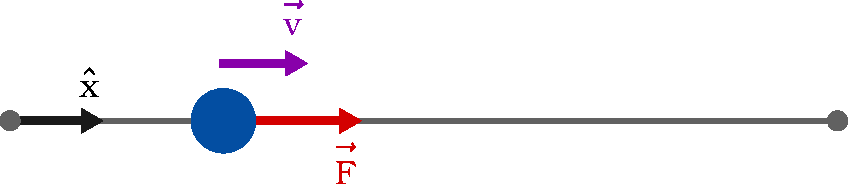
\includegraphics[width=0.72\textwidth]{Cap3/figuras/movimento-simples.pdf}
    \caption{Diagrama de forças no movimento simples}
    \label{fig:movimento-simples}
\end{figure}

\begin{equation}
    \mathbf{x} = \begin{bmatrix}
        s_x \\
        v_x
    \end{bmatrix},
    \qquad
    \mathbf{u} = \begin{bmatrix}
        F
    \end{bmatrix},
    \qquad
    \dot{\mathbf{x}} = \begin{bmatrix}
        v \\
        F/m
    \end{bmatrix},
    \label{eq:movimento-simples}
\end{equation}

\begin{equation}
    J = \int_{t_0}^{t_f} \left[ F^2 \right] dt.
    \label{eq:movimento-simples-J}
\end{equation}

\subsection{Braquistócrona}
\label{subsec:braquistocrona}

O problema da braquistócrona, proposto por Johann Bernoulli em 1696, consiste em encontrar a curva que minimiza o tempo de descida de uma partícula entre dois pontos sob ação da gravidade, desconsiderando o atrito. O nome vem do grego ``\textit{brachistos}'' (mais curto) e ``\textit{chronos}'' (tempo).

Embora possa parecer intuitivo que a linha reta seria a solução ótima por ser o caminho mais curto entre dois pontos, a solução do problema é uma curva cicloide. Isso ocorre porque, apesar do caminho ser mais longo, a partícula consegue atingir velocidades maiores ao longo da trajetória devido à maior inclinação inicial, resultando em um tempo total menor.

Este problema é considerado um dos marcos históricos do cálculo variacional e da otimização de trajetória, tendo sido resolvido por grandes matemáticos como Newton, Leibniz e o próprio Bernoulli. Sua solução analítica pode ser obtida através do princípio de Hamilton, mas aqui será utilizada uma abordagem numérica através da colocação trapezoidal.

Para modelizar o problema, considere um ponto material de massa $m$ sob ação da gravidade, que se move entre dois pontos fixos, conforme ilustrado na Figura \ref{fig:braquistocrona}. Apesar de sabermos que se trata de uma descida, a figura ilustra o ponto final com posições positivas ($s_x,f > 0$ e $s_y,f > 0$), de modo que o ângulo de inclinação da trajetória seja positivo e que se evitem problemas com convenções de sinais.

Utilizam-se as posições horizontal e vertical da partícula, além do valor absoluto da velocidade, como variáveis de estado e o ângulo de inclinação da trajetória como variável de controle. O vetor estado, o vetor controle e a dinâmica do sistema são descritos pelas Equações \ref{eq:braquistocrona}.

Por fim, o problema consiste em encontrar a trajetória que minimiza o tempo de descida entre dois pontos, conforme Equação \ref{eq:braquistocrona-J}.

\begin{figure}[H]
    \centering
    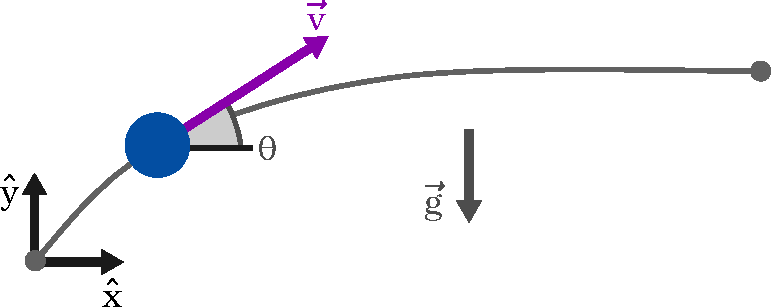
\includegraphics[width=0.72\textwidth]{Cap3/figuras/brachistochrone.pdf}
    \caption{Diagrama de forças no braquistócrona}
    \label{fig:braquistocrona}
\end{figure}

\begin{equation}
    \mathbf{x} = \begin{bmatrix}
        s_x \\
        s_y \\
        v
    \end{bmatrix},
    \qquad
    \mathbf{u} = \begin{bmatrix}
        \theta
    \end{bmatrix},
    \qquad
    \dot{\mathbf{x}} = \begin{bmatrix}
        v \cos(\theta) \\
        v \sin(\theta) \\
        -g \sin(\theta)
    \end{bmatrix},
    \label{eq:braquistocrona}
\end{equation}

\begin{equation}
    J = t_f.
    \label{eq:braquistocrona-J}
\end{equation}


\subsection{Trajetória de subida de eVTOL}
\label{subsec:evtol}

Por fim, apresenta-se o problema descrito em \cite{costa_otimizacao_2023}, que consiste em encontrar a trajetória de subida que minimize o consumo energético de um veículo multirrotor. Para modelar o problema, as variáveis de decisão utilizadas foram as posições $[s_x, s_y]$, velocidades $[v_x, v_y]$, energia total da bateria utilizada $E$ e comandos de tração dos rotores $[T_x, T_y]$, descritos pelas Equações \ref{eq:evtol}.

\begin{equation}
    \mathbf{x} = \begin{bmatrix}
        s_x \\
        s_y \\
        v_x \\
        v_y \\
        E
    \end{bmatrix},
    \qquad
    \mathbf{u} = \begin{bmatrix}
        T_x \\
        T_y
    \end{bmatrix},
    \label{eq:evtol}
\end{equation}

\begin{figure}[H]
    \centering
    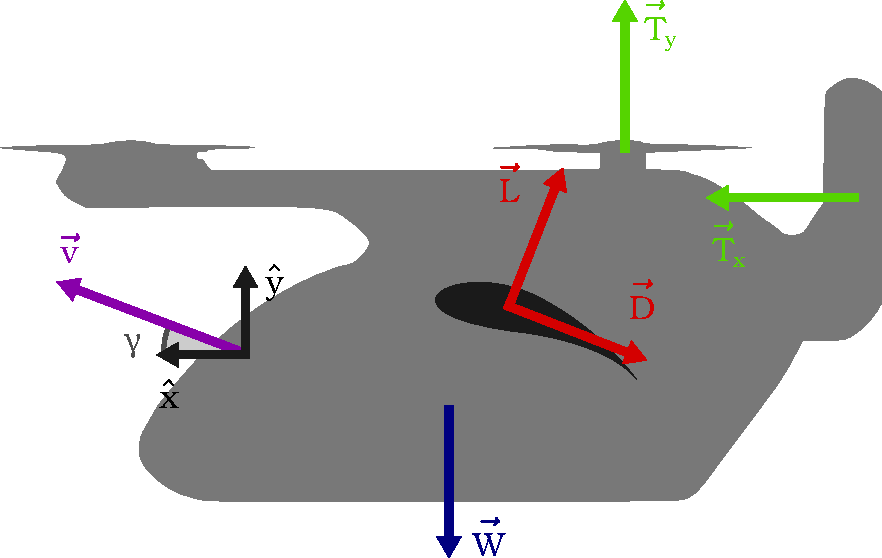
\includegraphics[width=0.72\textwidth]{Cap3/figuras/eVTOL.pdf}
    \caption{Diagrama de forças no eVTOL}
    \label{fig:evtol-forças}
\end{figure}

Conforme a Figura \ref{fig:evtol-forças}, a dinâmica do sistema pode ser descrita pelas Equações \ref{eq:evtol-dinamica}.

\begin{equation}
\begin{aligned}
    m\ddot{p}_x &= F_x = T_x - D(\mathbf{v}) \cos(\gamma) - L(\mathbf{v}) \sin(\gamma) \\
    m\ddot{p}_y &= F_y = T_y - D(\mathbf{v}) \sin(\gamma) + L(\mathbf{v}) \cos(\gamma) - mg,
\end{aligned}
\label{eq:evtol-dinamica}
\end{equation}

\noindent de modo que as restrições diferenciais escrevem-se

\begin{equation}
\begin{aligned}
    \dot{s}_x &= v_x \\
    \dot{s}_y &= v_y \\
    \dot{v}_x &= \dfrac{1}{m} F_x \\
    \dot{v}_y &= \dfrac{1}{m} F_y,
\end{aligned},
\qquad
\begin{aligned}
    \dot{E}
    &= P_{total} \\
    &=
    \begin{aligned}
        &\left( 2 P_{ind,rotor,x} (1 + \chi) + T_x |\mathbf{v}| \cos(-\gamma) \right) \\
        &+ \left( 4 P_{ind,rotor,y} (1 + \chi) + T_y |\mathbf{v}| \sin(-\gamma) \right).
    \end{aligned}
\end{aligned}
\label{eq:evtol-restricoes-diferenciais}
\end{equation}


Para finalizar a formulação do PCO, dado que se almeja o consumo mínimo da bateria, define-se a função objetivo como

\begin{equation}
    J = E_f.
    \label{eq:evtol-J}
\end{equation}

